\documentclass[12pt, titlepage]{article}

\usepackage{fullpage}
\usepackage[round]{natbib}
\usepackage{multirow}
\usepackage{booktabs}
\usepackage{tabularx}
\usepackage{graphicx}
\usepackage{float}
\usepackage{hyperref}
%\usepackage{tabularray}
\hypersetup{
    colorlinks,
    citecolor=blue,
    filecolor=black,
    linkcolor=red,
    urlcolor=blue
}

%% Comments

\usepackage{color}

\newif\ifcomments\commentstrue %displays comments
%\newif\ifcomments\commentsfalse %so that comments do not display

\ifcomments
\newcommand{\authornote}[3]{\textcolor{#1}{[#3 ---#2]}}
\newcommand{\todo}[1]{\textcolor{red}{[TODO: #1]}}
\else
\newcommand{\authornote}[3]{}
\newcommand{\todo}[1]{}
\fi

\newcommand{\wss}[1]{\authornote{blue}{SS}{#1}} 
\newcommand{\plt}[1]{\authornote{magenta}{TPLT}{#1}} %For explanation of the template
\newcommand{\an}[1]{\authornote{cyan}{Author}{#1}}
%% Common Parts

\newcommand{\progname}{ProgName} % PUT YOUR PROGRAM NAME HERE
\newcommand{\authname}{Team \#, Team Name
\\ Student 1 name and macid
\\ Student 2 name and macid
\\ Student 3 name and macid
\\ Student 4 name and macid} % AUTHOR NAMES                  

\usepackage{hyperref}
    \hypersetup{colorlinks=true, linkcolor=blue, citecolor=blue, filecolor=blue,
                urlcolor=blue, unicode=false}
    \urlstyle{same}
                                


\newcounter{acnum}
\newcommand{\actheacnum}{AC\theacnum}
\newcommand{\acref}[1]{AC\ref{#1}}

\newcounter{ucnum}
\newcommand{\uctheucnum}{UC\theucnum}
\newcommand{\uref}[1]{UC\ref{#1}}

\newcounter{mnum}
\newcommand{\mthemnum}{M\themnum}
\newcommand{\mref}[1]{M\ref{#1}}

\begin{document}

\title{System Design for Digital Twin Forest} 
\author{Team 8, Forest Mirror\\Yichen Jiang\\ Bowen Zhang\\ Jiacheng Wu\\ Junhong Chen\\ Tingyu Shi}

\date{\today}

\maketitle

\pagenumbering{roman}

\section{Revision History}

\begin{tabularx}{\textwidth}{p{3cm}p{2cm}X}
\toprule {\bf Date} & {\bf Version} & {\bf Notes}\\
\midrule
January 5 & 1.0 & Work Delivery\\
\hline
January 10 & 2.0 & Revision 0\\
\hline
April 2 & 3.0 & Final Version\\
\bottomrule
\end{tabularx}

\newpage

\section{Reference Material}

This section records information for easy reference.

\subsection{Abbreviations and Acronyms}

\renewcommand{\arraystretch}{1.2}
\begin{tabular}{l l} 
  \toprule		
  \textbf{symbol} & \textbf{description}\\
  \midrule 
  FR & Functional Requirement\\
  MG & Module Guide \\
  MIS &  Module Interface Specification\\
  SRS & Software Requirements Specification\\
  UI & User Interface\\
  V\&V & Verification and Validation\\
 
  
  
  \bottomrule
\end{tabular}\\

\newpage

\tableofcontents

\newpage

\listoftables

\listoffigures

\newpage

\pagenumbering{arabic}

\section{Introduction}

This document is the system design of the project Digital
Twin Forest. A digital twin forest is a virtual 
representation of the natural world, specifically a real 
forest in our project. The detailed introduction of our
project can be found in our \href{https://github.com/wuj187/DigitalTwinCAS/blob/main/docs/ProblemStatementAndGoals/ProblemStatement.pdf}{Problem Statement} and \href{https://github.com/wuj187/DigitalTwinCAS/blob/main/docs/SRS/SRS.pdf}{SRS}.

\section{Purpose}

Our system has the following three main purposes:
\begin{itemize}
\item A virtual representation of the real forest,
allowing monitoring and analyzing from a distance.
\item Visualizing important data related to scientific 
research and decision-making. For the environment, 
important data include temperature, humidity, etc. 
For tree parameters, important data include tree density,
tree heights, tree diameters, etc.
\item A forest model that can change dynamically 
according to the modification of the data.
\end{itemize}

\noindent The purpose of this design document is to
illustrate and verify the decomposition of the system 
into different components. This document will show 
the general idea of how the team is going to 
implement the application, and guarantee the design
meet all functional and non-functional requirements. 
In addition, it provides an overview of the system behavior. We have also completed  \href{https://github.com/wuj187/DigitalTwinCAS/blob/main/docs/Design/MG/MG.pdf}{Module Guide} and  \href{https://github.com/wuj187/DigitalTwinCAS/blob/main/docs/Design/MIS/MIS.pdf}{Module Interface 
Spcification}.

\section{Scope}

The system includes JSON files which are used to 
store the forest data, a 3D model of the terrain and 
the virtual forest, and a graphical user interface. 
A scene manager is used to control user behaviors, 
the users can interact with the UI to read and modify
the data. The users will be able to control the 
camera and view the forest from different 
perspectives.

\subsection{Context Diagram}
\begin{figure}[H]
    \centering
    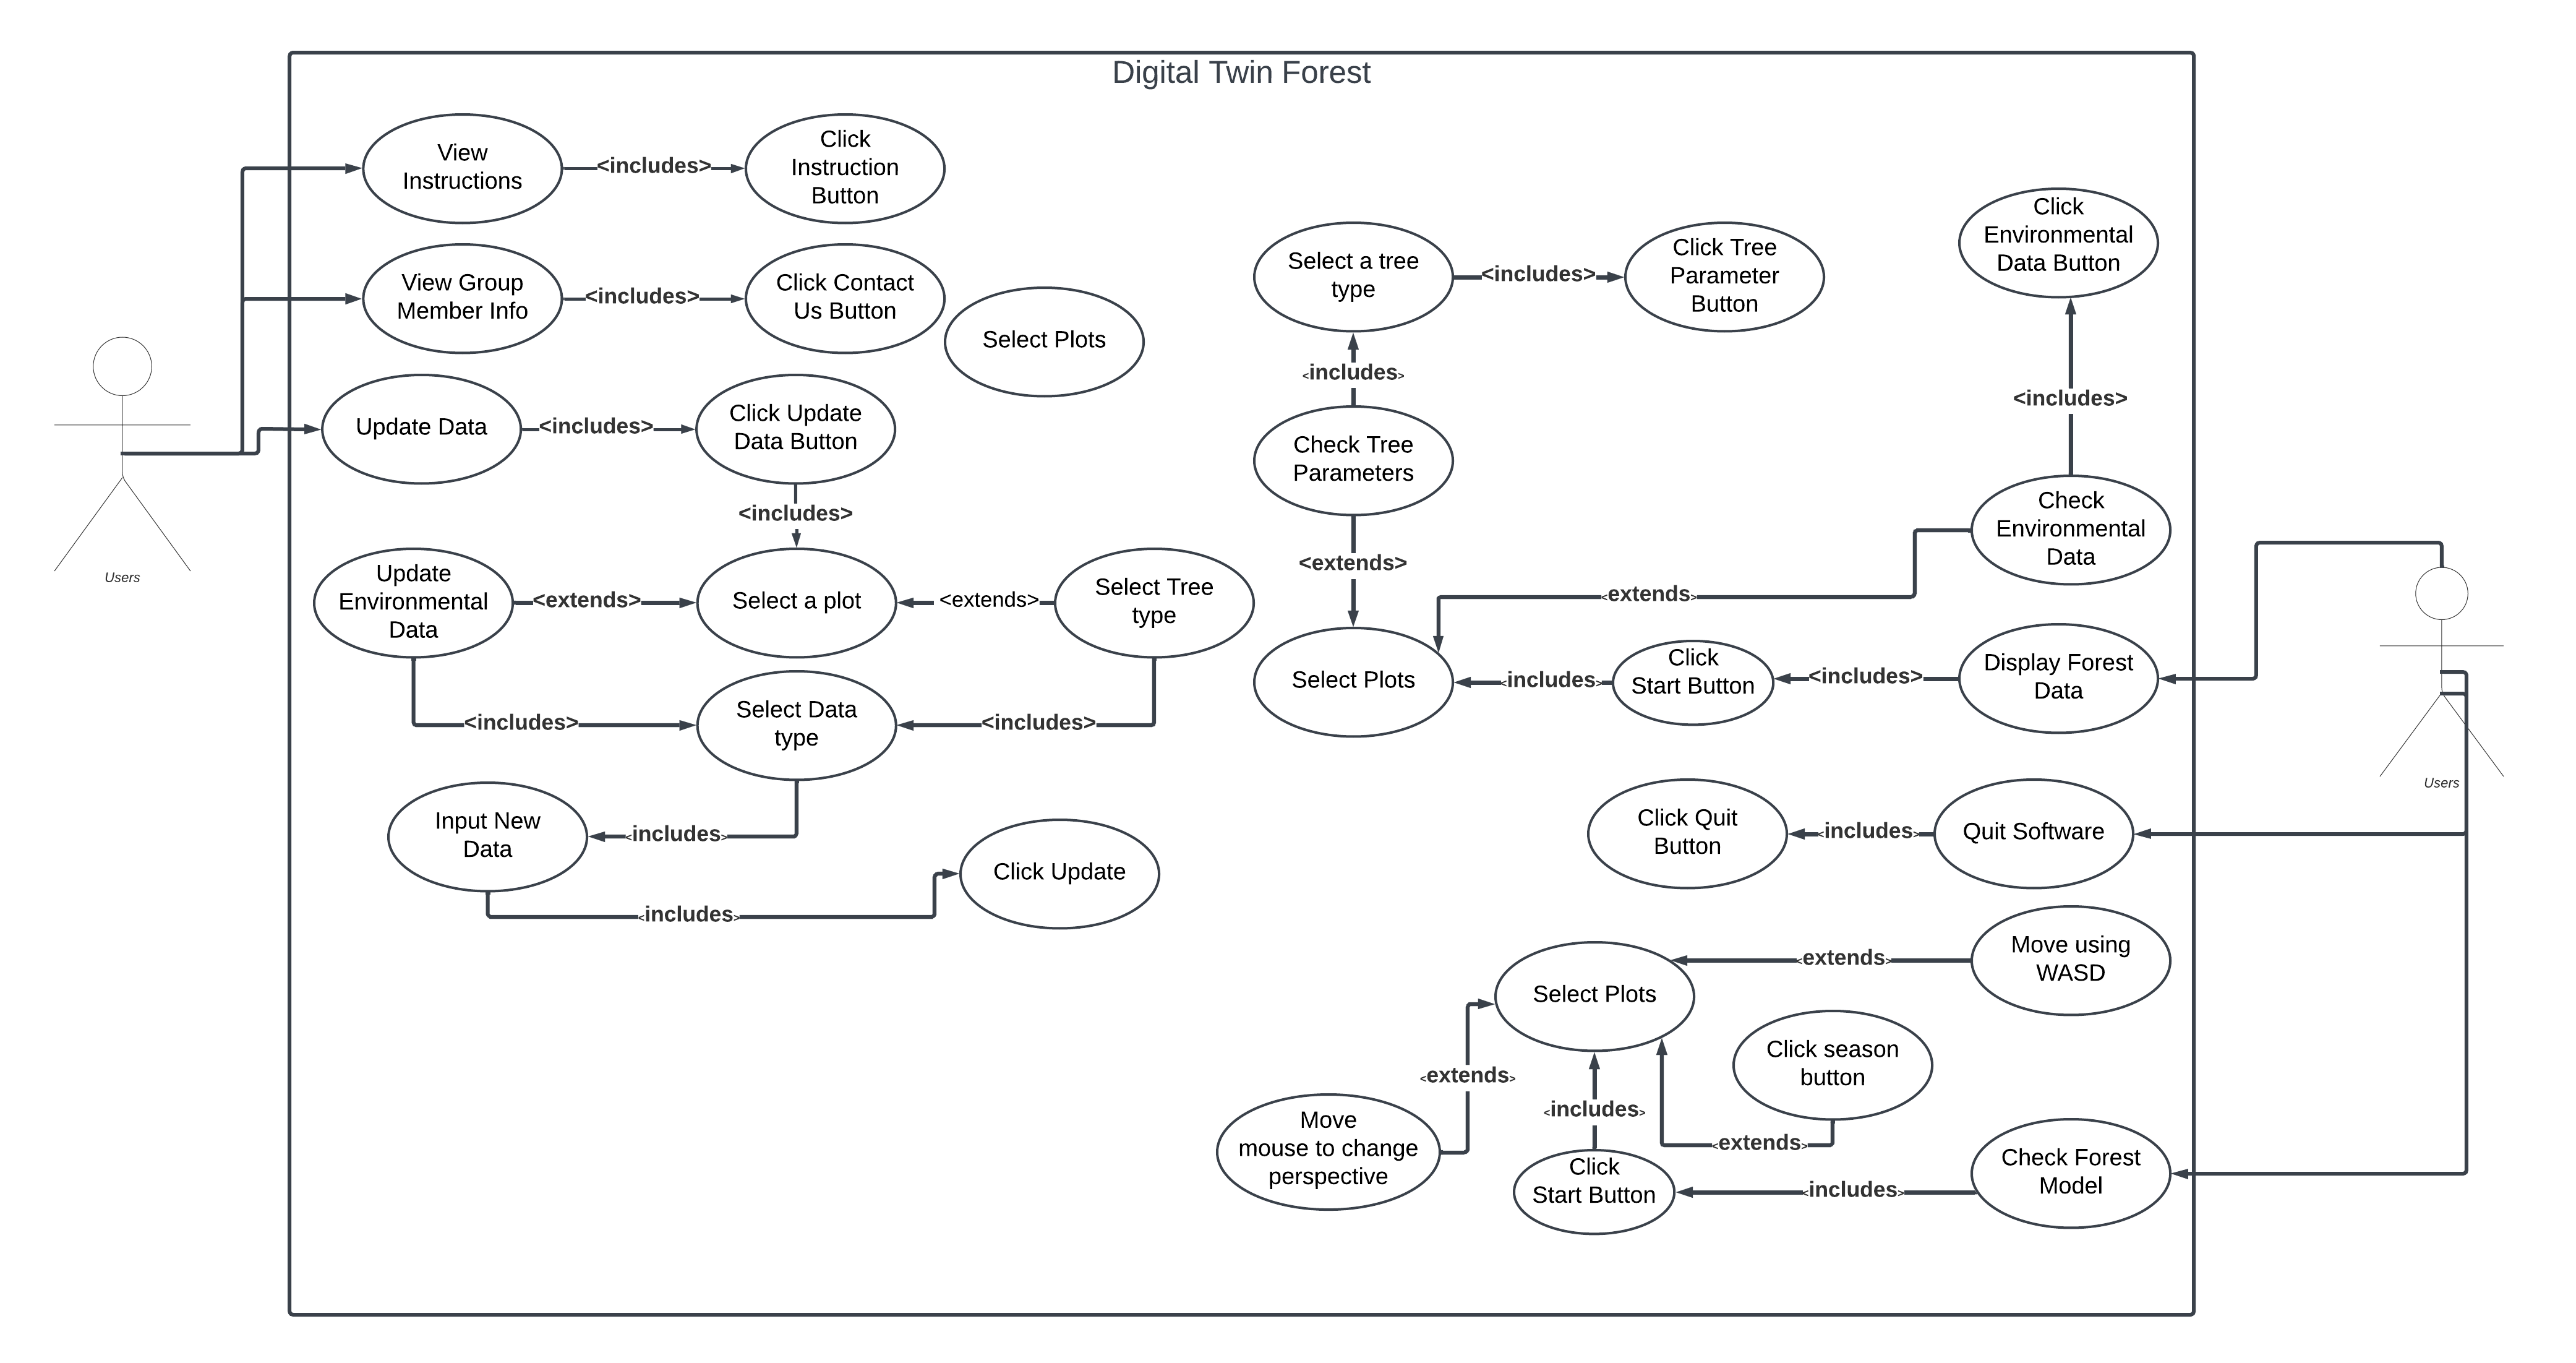
\includegraphics[scale=0.28]{SysDesPic/Use_Case.png}
    \caption{Context Diagram}
    \label{usecase}
\end{figure}

\subsection{Assumptions}
\begin{itemize}
    \item The generated model will only use the average data and will not be exactly the same with the real forest.\\
    Rationale: The parametric modeling and sampled data save a lot of implementation time and computing resources. And for now, the developers can only access to the average data from the supervisor's lab. 
    \item The users have the right to update the data with any value and the correct data type locally. \\
    Rationale: The users might use the product to visualize the forest with parameters which may differ from the reality. They would be allowed to update the data even if the data do not completely correspond with the reality. Therefore, the product would not provide solutions to check if the data are accurate.\\
    \item The system will only be installed on a personal computer.\\
    Rationale: The mainstream scenarios of this product being used are on the personal computers (either by forest owners or the environmental scientists). The product is designed and developed corresponding to these scenarios. 
    
\end{itemize}

\section{Project Overview}

\subsection{Normal Behaviour}
Digital Twin Forest is a software application that combines virtual forests with real-world data to provide users with comprehensive information about real-world forests. The application visualizes this data for users, including overall environmental data for each plot and detailed information about each type of trees in it. This would assist forest owners in making economic decisions without physically visiting the forest, as well as aid scientists in research such as climate change and environmental analysis. \\

\noindent When the application is launched, a main page will appear, where users can click on various buttons to perform different actions. The ``Start" button loads the models and data, allowing users to view the virtual forests and their associated data. The ``Instruction" and "Contact Us" buttons lead users to the instruction and contact pages respectively. Within the instruction and contact pages, the ``Back" button will take users back to the main page when users click on it. The ``Quit" button on the main page allows users to exit the application.\\


\noindent On the model page, data about each plot and each type of trees within it can be displayed or hidden by clicking on the ``Show Environmental Data" and ``Show Overall Tree Parameters" buttons. By clicking the switch button on the panel that shows environmental data, the panel should switch between environmental data and a pie chart displaying the percentage of each types of tree. By clicking the switch button on the panel that shows tree parameters, the panel should switch between tree parameters and leaf information. When different plots are selected, the data displayed will change to reflect that specific plot. The camera's perspective in the model changes as the user moves his mouse, and the camera's position can be adjusted as the user presses the \textbf{WASD} keys. By pressing \textbf{P} key, the movement of perspective should disconnect with the mouse. Pressing \textbf{P} again should reconnect the movement of perspective and the mouse. By pressing \textbf{C}, the position of the cursor should come to the center of the screen. The ``Back" button will take users back to the main page when users click on it.\\

\noindent The ``Update Data" button on the main page will take users to a page where they can modify tree parameters and environmental data. The "Select Plot" button should display a drop-down menu which allows the users to select plot to update data after clicked. After a plot is selected, the "Update Environmental Data" should allow users to choose which data to be updated after clicked. And the "Update Tree Parameters" button should allow users to choose the data of which type of trees to be updated after clicked. After choosing a certain attribute of either environmental data or a specific type of trees, an input box should show, indicate the original value of the chosen attribute, and allow the users to input the new value. After users enter the new data, it will replace the old data and display on the screen.
The ``Back" button will take users back to the main page when users click on it.

\subsection{Undesired Event Handling}

Users can manually adjust the data stored in the application. However, if users mistype and accidentally enter data with unexpected data type, an error would occur. To avoid this, a data validation function was added to this application, enabling the system verify whether the data type is valid. If the data type is not valid, the application will display an error message to inform users that the data entered is not valid, reminding them to re-enter the data. The validation process would repeat until valid data is entered and successfully updated. 

\newpage

\subsection{Component Diagram}

We used MVC to implement our system, so the following three diagrams show the relationships of
modules within Model modules, Viewer modules, and Controller modules.

\begin{figure}[H]
\caption{Relationships between Model modules}
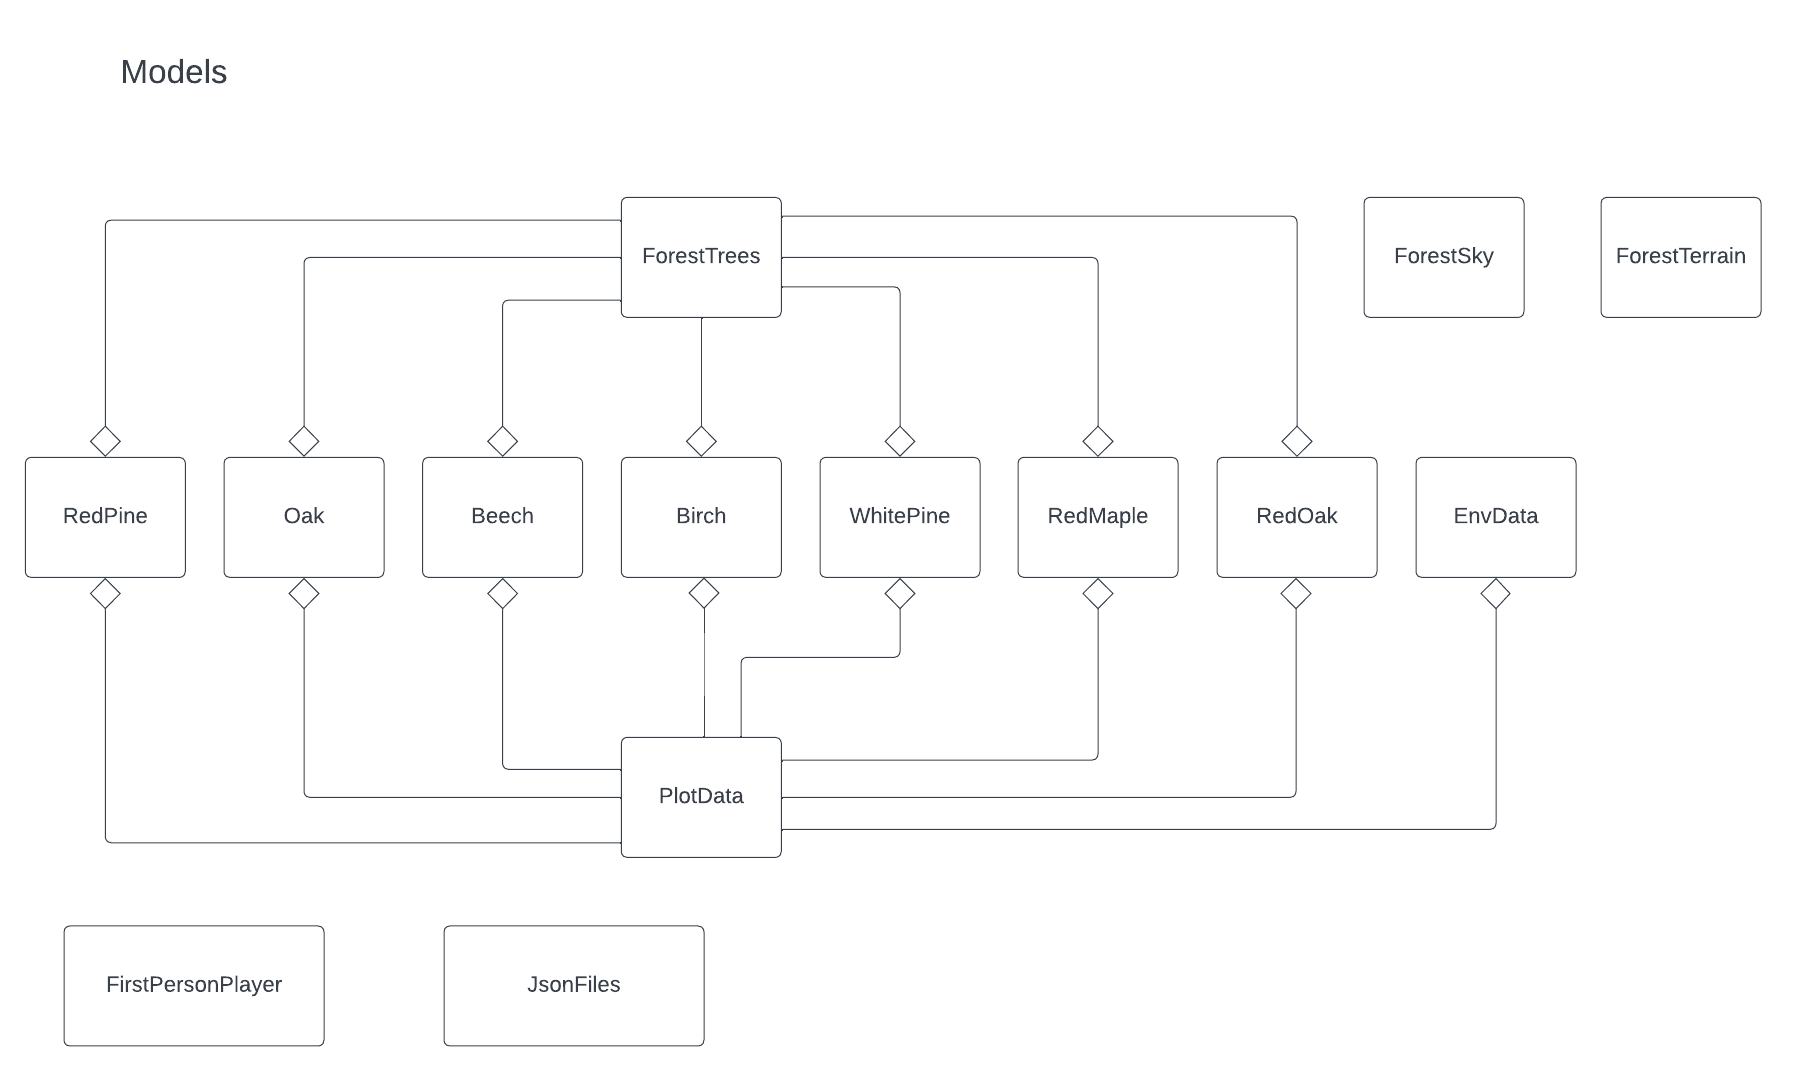
\includegraphics[scale=0.65]{SysDesPic/Model-Modules.png}
\end{figure}

\noindent The structure of Model modules is designed to adapt the method of storing the data in JSON files. 

\newpage

\begin{figure}[H]
\caption{Relationships between Viewer modules}
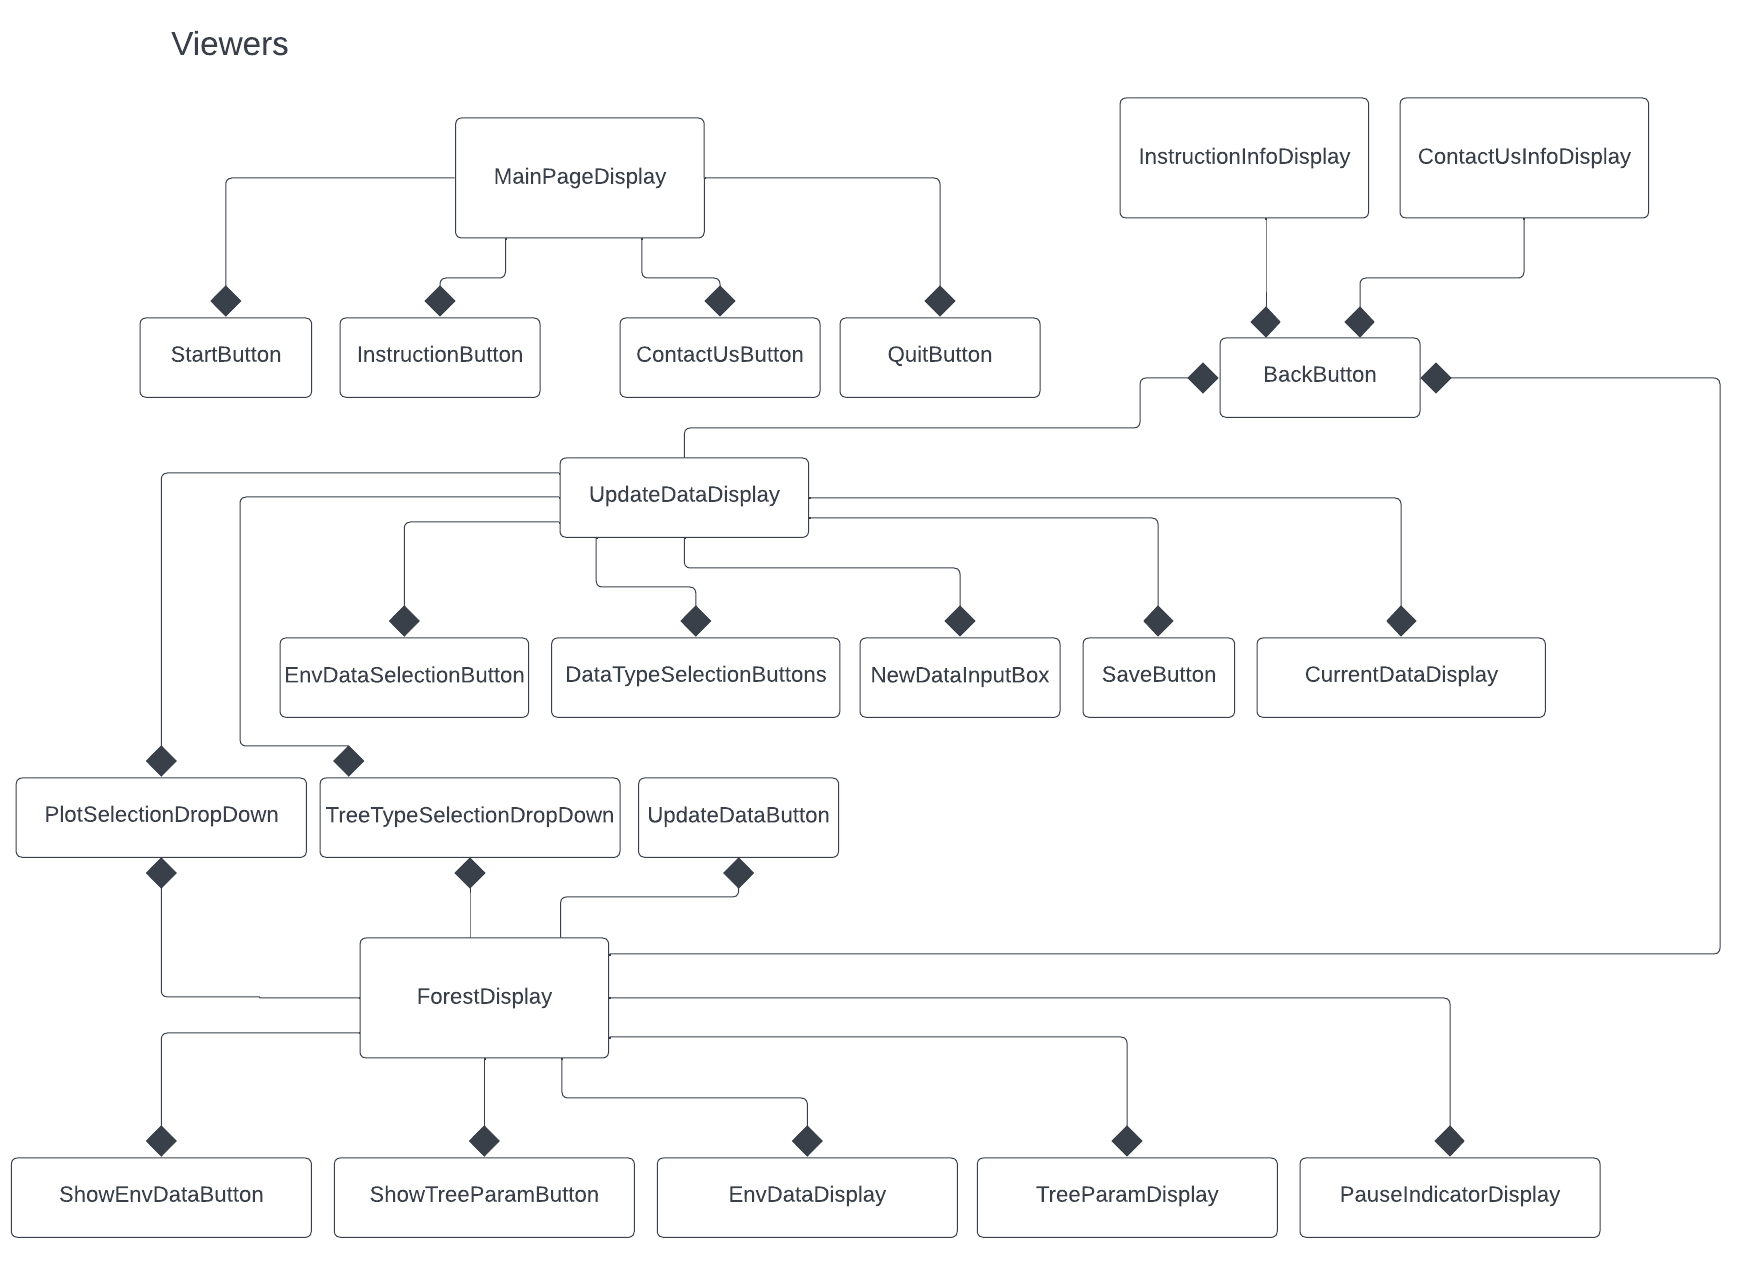
\includegraphics[scale=0.65]{SysDesPic/Viewer-Modules.png}
\end{figure}

\newpage

\begin{figure}[H]
\caption{Relationships between Controller modules}
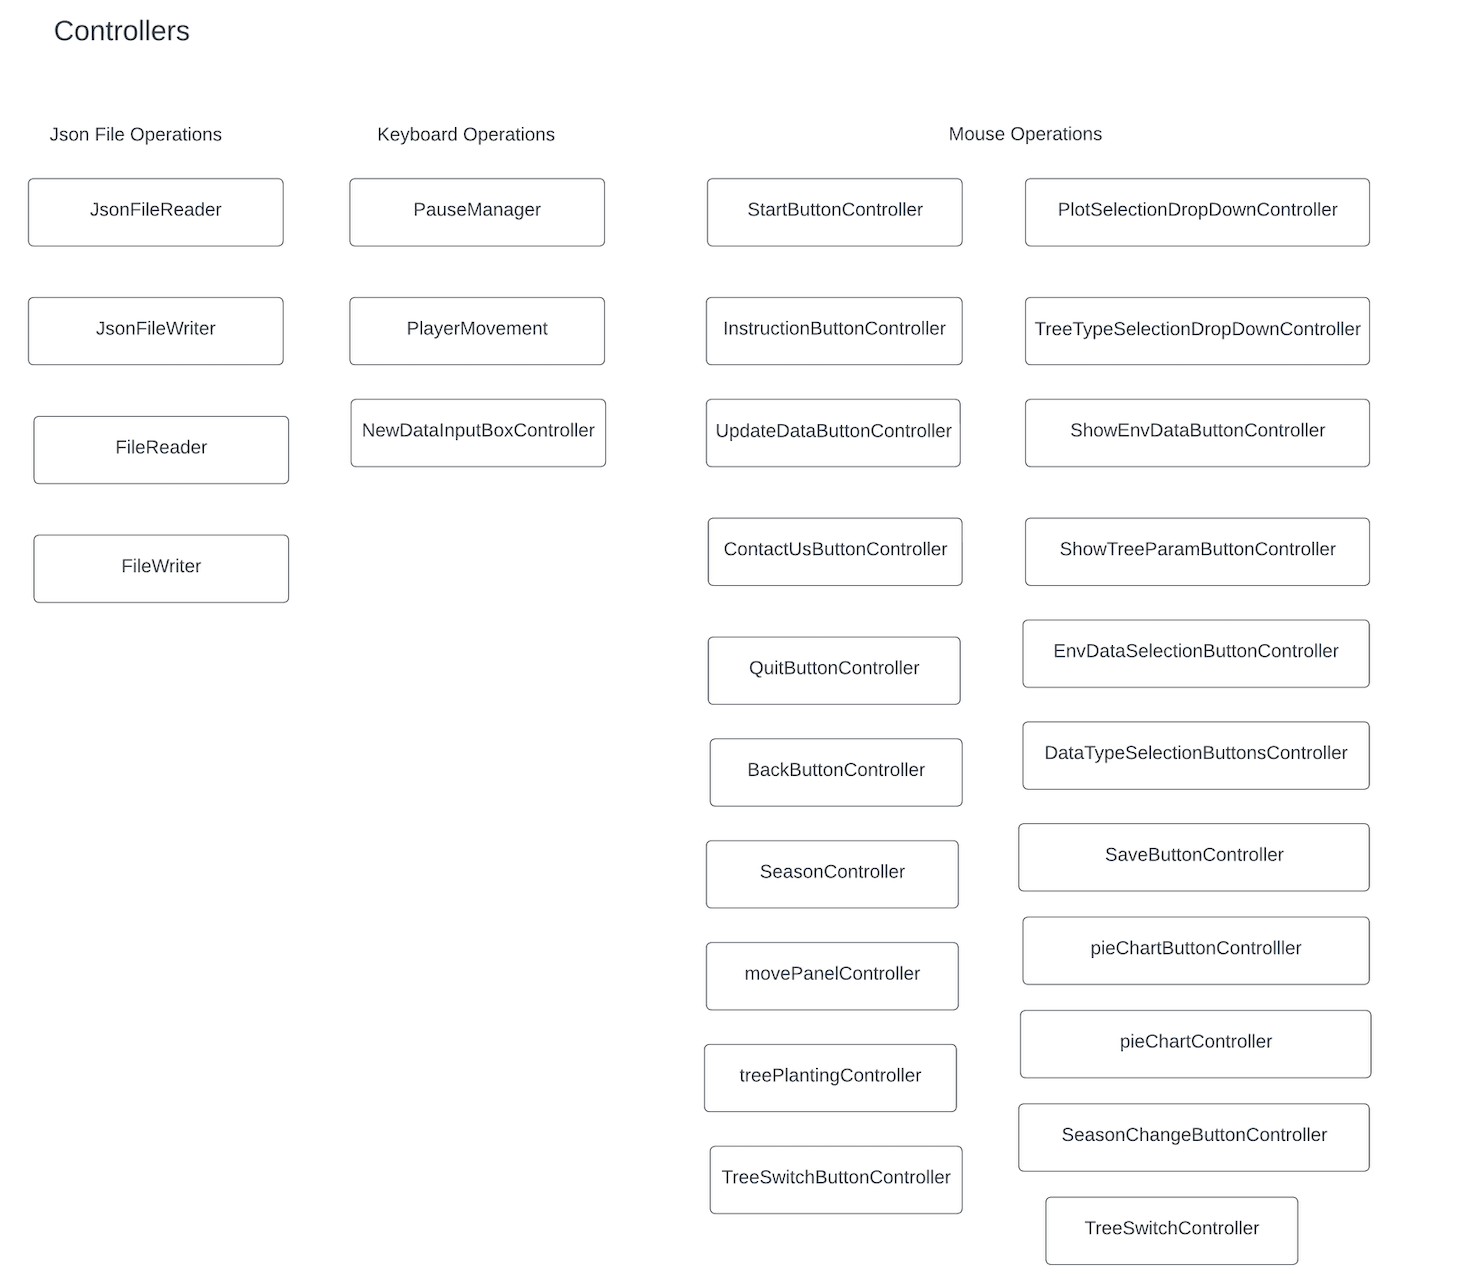
\includegraphics[scale=0.65]{SysDesPic/Controller-Modules.png}
\end{figure}

\newpage

\subsection{Connection Between Requirements and Design}

\label{SecConnection}

The intention of this section is to document decisions that are made
  ``between'' the requirements and the design.  To satisfy some requirements,
  design decisions need to be made.  Rather than make these decisions implicit,
  they are explicitly recorded here.  For instance, if a program has security
  requirements, a specific design decision may be made to satisfy those
  requirements with a password.\\
  
\noindent All requirements about data storage(SR1.2, SR2.3) - The system uses JSON files to store data. It is not appropriate to allow users to directly modify the data in these files by hand because it does not meet requirements SR1.2 and SR2.3, and it can also lead to problems such as accidentally deleting the entire file or deleting the wrong content. To address this, functions for reading and writing JSON files have been developed and linked to the ``Update Data" page, which provides an interface for users to update the data.\\

\noindent All requirements about the user interface of environmental data and tree parameters (FR4, FR5, FR6, FR7) - The ``Show Environmental Data" button and the ``Show Overall Tree Parameters" button on the upper-left and upper-right corners of the screen allow users to show and hide the environmental data and the tree parameters. When users click on these buttons, the environmental data and tree parameters will be shown on the two sides of the screen, without interrupting the user's view of the virtual forest. There is a function in the back-end code that takes a Boolean value to determine whether the data is shown or not, and this function is bound to these two buttons. If users want to hide the data, they can click on the buttons again to hide the data. In the middle of the upper edge of the screen, there is a button where users can select which plot they want to see. As users select a different plot, the corresponding environmental data and tree parameters for that specific plot will be displayed.\\

\noindent All requirements of the instruction page and start button (FR1, FR3) - A ``Start" button and an ``Instructions" button have been designed, programmed, and placed on the main page, allowing users to enter the virtual forest and access the instructions page.\\

\noindent Requirement about quitting the application (FR11) - A ``Quit" button has been designed, programmed, and placed on the main page, allowing users to exit the application as users click on it. On the virtual forest page, a "Back" button has been designed the programmed to that users can quit the virtual forest page and go back to the main page.\\

\noindent Requirement about the update data page (FR12) - An ``Update data" button has been designed and placed on the home page to allow users to enter the page where they can modify and update the data.\\

\noindent All requirements about user movement (FR8, FR9) - The code uses a \textit{Vector} data type variable to store and calculate the direction of the camera's movement and calls the \textit{Move} function to enable the camera's movement. The code records the axis of the mouse with \textit{Input.GetAxis} functions, and uses \textit{Quaternion.Euler} and \textit{Transform.Rotate} functions to calculate the movement of the mouse. Therefore, Users can press the \textbf{WASD} keys to move the camera and move their mouse to adjust the camera's perspective. As users move the perspective of the camera up and press the \textbf{W} key, they can zoom out of the virtual forest. On the contrary, by moving the perspective down and pressing the \textbf{S} key, they can zoom in on the virtual forest. The initial position of the camera is set above the forest, so users can see a full view of the overall digital twin forest.

\section{System Variables}

This section is for Mechatronics projects. We would not include this section in this document. 

\subsection{Monitored Variables}

\subsection{Controlled Variables}

\subsection{Constants Variables}

\section{User Interfaces}


We designed our user interface based on the users' need to organize data and view data hierarchically. The detailed design is described below, and we attached the manuscript of the design in Appendix A.\\

\noindent When the product is launched, a welcome page is displayed, with buttons of start, contact us, instruction, and quit. The background of the welcome page is a picture of a forest, which corresponds to the function of our product. In the pages of contact us and instruction, we use the same background to make the appearance consistent. \\

\noindent The users can click start to launch the model or click quit to terminate the program. When the model is launched, the product displays a model of the target forest, with a view of a height of about two meters above the ground. The users can use the mouse to change the perspective and use the keyboard \textbf{WASD} to move the camera within the model. The model is parametrically generated and highly reappears the real view in the target forest. \\

\noindent Meanwhile, there are three buttons on the top of the screen. The first one shows the current plot. The users can click it to change the plot or show the overall data of the forest. If this button is clicked, a drop-down menu shows up and displays all possible options. The second one is seasonal change button, showing the current season in the model. The users can click it to switch between summer and winter. The third one shows the type of trees selected for the tree parameters panel. The users can click it to change the type of trees. If this button is clicked, a drop-down menu would show up and display all possible options. \\

\noindent On the upper left corner, there is a button which allows the user to access or hide the environmental data of the selected plot. The data would be displayed in a floating panel, which isolates the data and the model. And on the upper right corner, there is a similar button for the tree parameters. When the users access to the tree parameters, there is another drop-down menu to categorize the data by the types of trees. \\

\noindent To avoid the sudden change of the camera direction when checking the data, the user can press \textbf{P} on the keyboard to pause the movement of the camera and press \textbf{P} again to resume. \\

\noindent In case the cursor is moved to the edge of the screen, the users can press \textbf{C} to move the cursor to the center of the screen. \\

\noindent With this design, the data required by the users will be firstly categorized by each plot and then by environment and tree parameters. The data can be organized in this way. The users can access to a certain part of the data. \\

\noindent In the main page, the users are allowed to modify some specific data by clicking an update button. After clicking it, the product will redirect to a new interface with choices of the serial number of the plot, then environmental data/ tree parameters and the tree type. After making all the choices, the interface displays all the possible data corresponding to the former choices. The user can read the old data, input the new data in this interface, and click ''Update" to do the modification. Modified data will show up on the model page right after this operation. After the modification, the users can click exit on the lower left corner to go back to the main page.\\

\noindent To exit the model, the users can click the button Back to go back to the main page. 


\section{Design of Hardware}

Most relevant for mechatronics projects. Show what will be acquired. Show what will be built, with detail on fabrication and materials. Include appendices as appropriate, possibly with sketches, drawings, CAD, etc.

\section{Design of Electrical Components}

Most relevant for mechatronics projects. Show what will be acquired. Show what will be built, with detail on fabrication and materials. Include appendices as appropriate, possibly with sketches, drawings, circuit diagrams, etc.

\section{Design of Communication Protocols}

If appropriate.

\section{Timeline}
\begin{itemize}
    \item January 10: Finish data storing modules (JSON files) with Dr. Gonsamo's lab members. The team will get the accurate forest data from the lab and start to implement the user interface. - All team members.
    \item January 15: Finish adding the user interface component. The team shall implement scripts to let the users read and write the forest data. - Tingyu Shi \& Jiacheng Wu.
    \item January 22: Finish modifying the modelling component by adding new species to the virtual forest. New models shall be added to the existing digital twin so that the number of species is the same with the accurate data. The virtual tree height and tree density shall also follow the measured data. - Bowen Zhang.
    \item February 5: Finish enough tests and verification before the revision 0 demonstration. The team will follow the V\&V plan to do manual and automated testings to guarantee the correctness of the system. - Yichen Jiang \& Junhong Chen
    \item February 6: Revision 0 Demonstration - All team members.
\end{itemize}
% \bibliographystyle {plainnat}
% \bibliography{../../../refs/References}

\newpage{}

\appendix

\section{User Interface}

\begin{figure}[H]
    \centering
    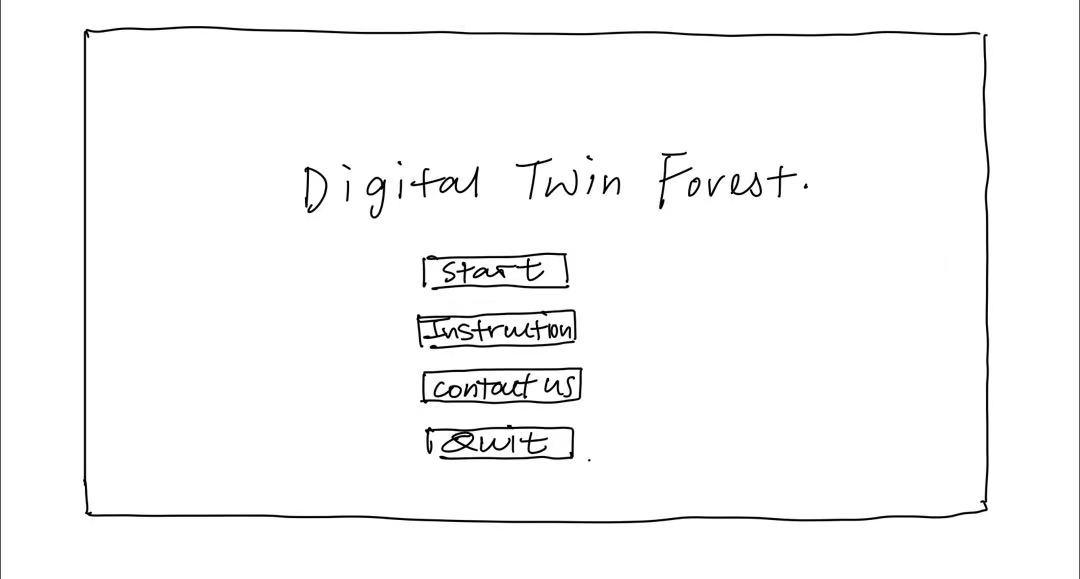
\includegraphics[scale=0.3]{SysDesPic/AppendixA-1.jpeg}
    \caption{Welcome Page}
\end{figure}

\begin{figure}[H]
    \centering
    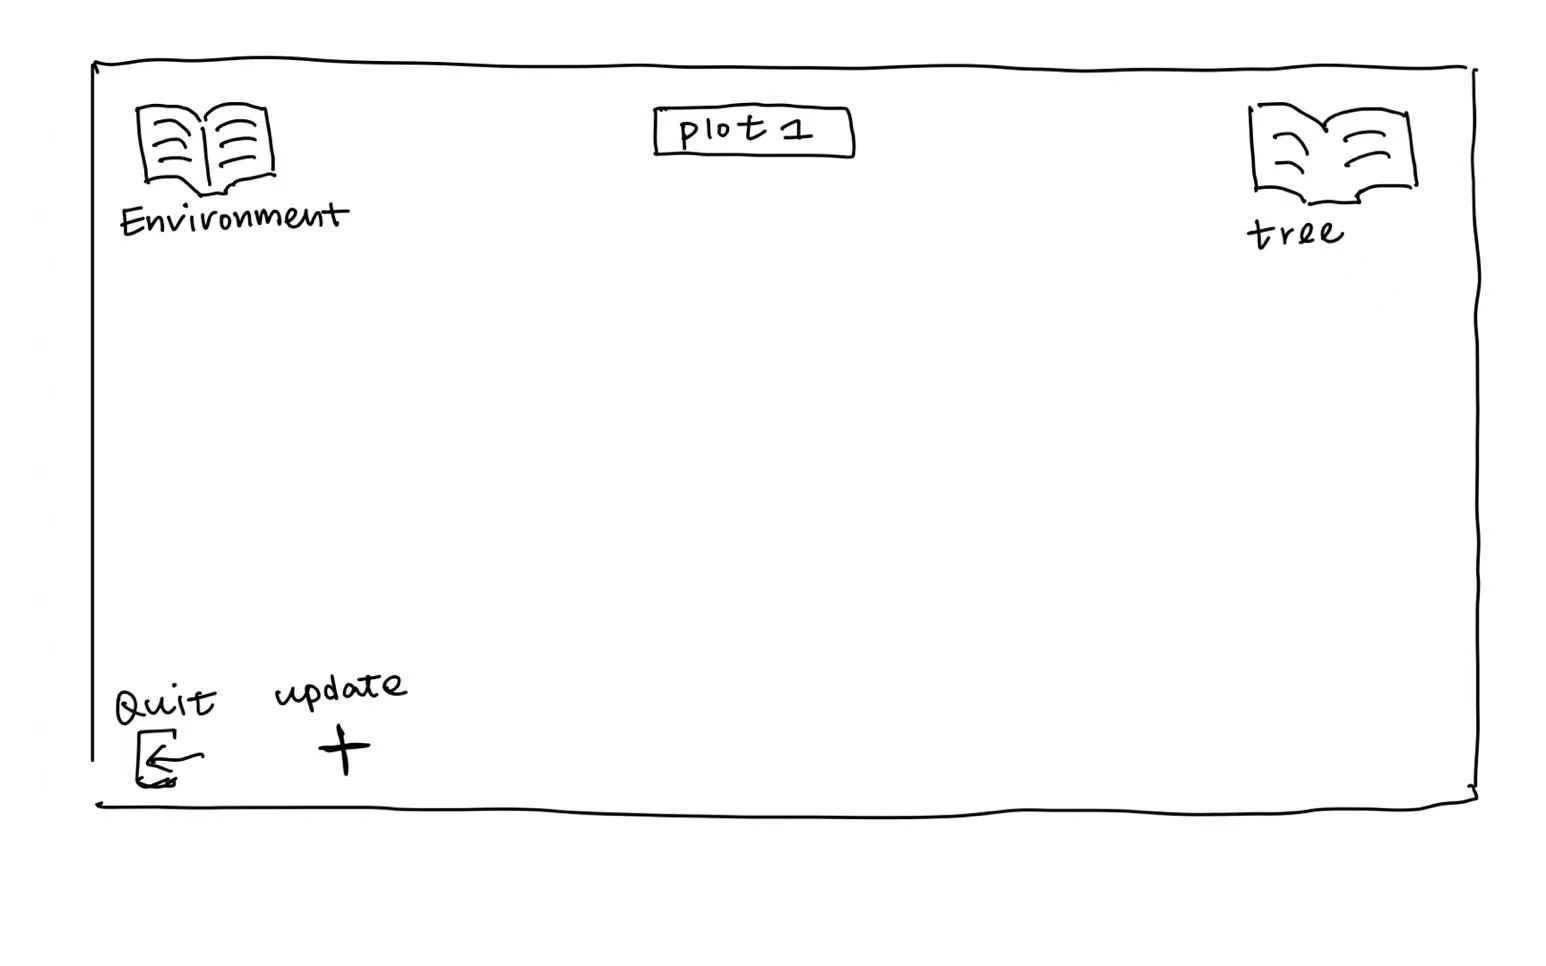
\includegraphics[scale=0.3]{SysDesPic/AppendixA-2.jpeg}
    \caption{Initialized Main Page}
\end{figure}

\begin{figure}[H]
    \centering
    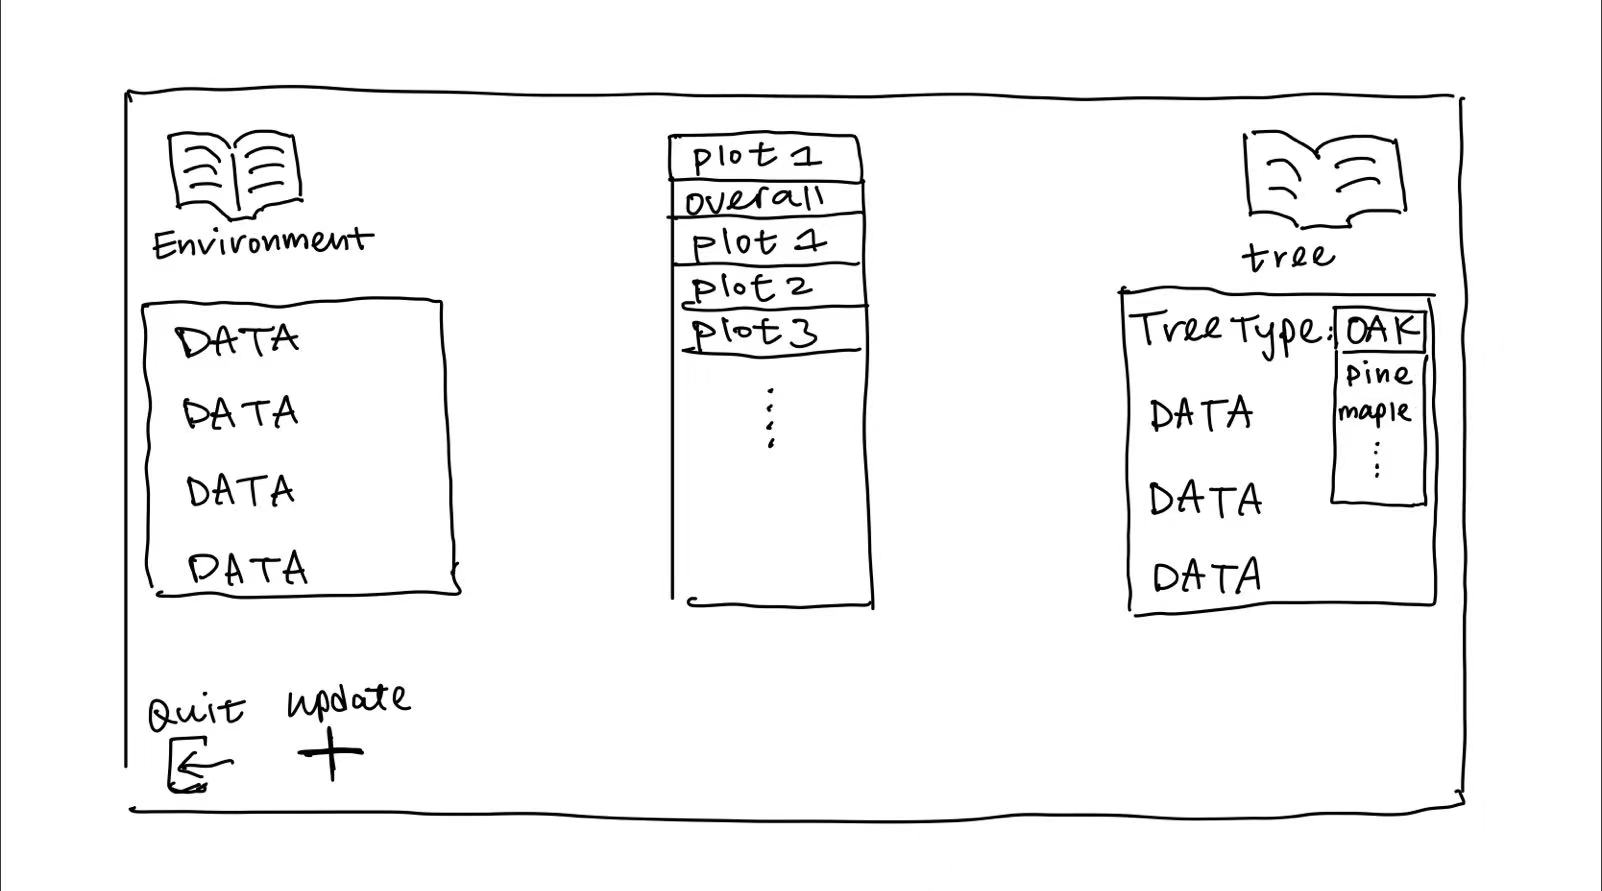
\includegraphics[scale=0.3]{SysDesPic/AppendixA-3.jpeg}
    \caption{Extended Main Page}
\end{figure}

\begin{figure}[H]
    \centering
    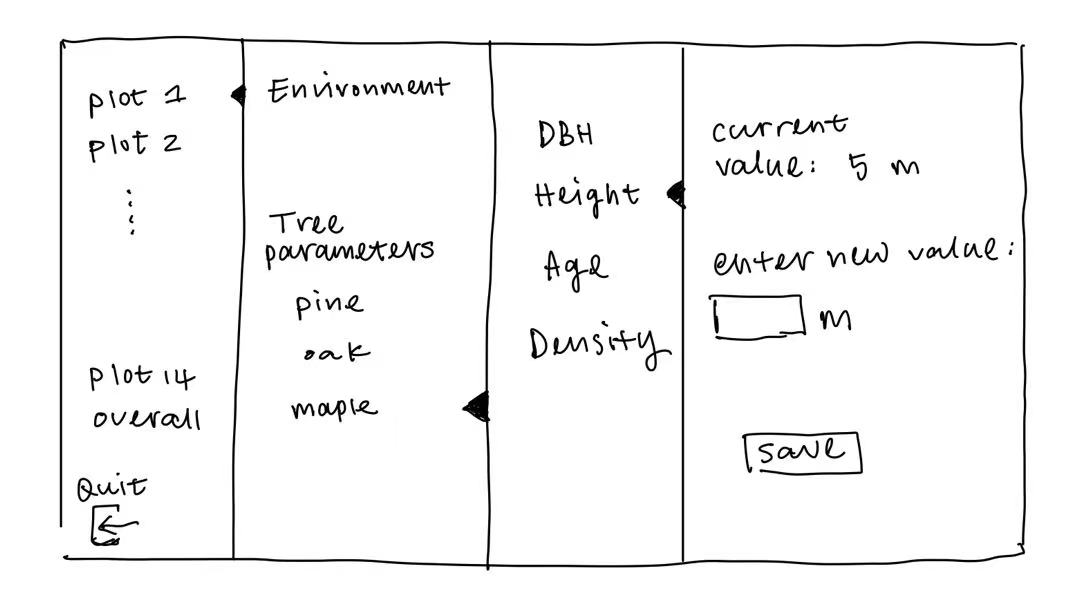
\includegraphics[scale=0.4]{SysDesPic/AppendixA-4.jpeg}
    \caption{Update Data Page}
\end{figure}


\section{Mechanical Hardware}

\section{Electrical Components}

\section{Communication Protocols}

\section{Reflection}

The information in this section will be used to evaluate the team members on the
graduate attribute of Problem Analysis and Design.  Please answer the following questions:

\begin{enumerate}
  \item What are the limitations of your solution?  Put another way, given
  unlimited resources, what could you do to make the project better? (LO\_ProbSolutions)
  \item Give a brief overview of other design solutions you considered.  What
  are the benefits and trade-offs of those other designs compared with the chosen
  design?  From all the potential options, why did you select documented design?
  (LO\_Explores)

\begin{itemize}
    \item Yichen\\ 
A limitation of our solution is that the model does not perfectly correspond to the target forest. With this limitation, any interaction with the model seems to be meaningless. This limitation leads to more limitations we currently have. We would love to implement some features based on the models originally, but we have to give these ideas up because of this limitation. For instance, we considered measuring the distance between two trees initially, but we found that it is impossible to reappear 100\% of the target forest using Unity with our budget and schedule, and measuring the distance between two trees in such a model does not make sense. If we could have more time and budget, or at least some advanced 3D scanning devices, we could give a better model with higher fidelity and therefore realize more features we came up with. \\

In the modelling phase, there were two alternatives. One is to use 3D scanning devices and cover the whole plot. The other one is parametric modelling, using the measured data provided by our supervisor and his research group. We also considered implementing some interactive features with the model, such as displaying more data about a specific tree if it is clicked, measuring the distance between two trees, etc. The benefits of these alternatives include showing the data more directly and intuitively, while the trade-off is that it has a high requirement for our model fidelity. And as mentioned above, the budget and schedule do not allow us to give a satisfying scanned model. Thus we chose the documented design. \\

Besides, in the feature of updating data, we considered letting our users directly modify the data files, while we currently choose to implement an independent page with a user interface to do so. The benefits of modifying data files include ease, less workload, and more freedom for our users. However, we think this alternative might require some professional programming knowledge, and it could be easier to get wrong and cause the crash of the whole product. Therefore, we chose the documented design with a complete user interface for updating data. \\
    
    \item Bowen\\
Limitations include the model, which could have a higher fidelity to the target forest, and the functions, which are limited by our method of modelling. To be specific, as we used parametric modelling, the model and target forest still have many differences. Therefore, the functions like measuring distance or interaction with specific trees cannot be realized on the top of a parametric generated model. The parametric generated model is indeed the best choice we have currently. We tried scanning the plot we would like to model using our mobile devices, but the outcome was not satisfying. An advanced scanning device could help, but it is over the budget, and we still need some time to learn about the new device. So if we have unlimited resources, the modelling method would be the first thing we would love to change. And there are more functions that can be realized on a perfectly modelled scene. \\

We considered the design based on the model, while the trade-off includes it highly depends on an accurate model, so we finally chose the documented design. And we considered letting our users directly modify the data file. The benefit is that it saves additional write operations when loading the model, and the trade-off is higher requirements for our users. We want a more consistent product, so chose the documented alternative over this one. Besides, we considered delivering 14 different models for the different plots, while as we used parametric modelling, the average data we used for modelling did not produce significant differences among the models. And this alternative will end up with a huge size of product. Therefore we just modified the corresponding data instead of changing all the models.


    
    \item Junhong

    The most significant limitation is the correlation between the model and the target forest. We failed to reappear all the details in the target forest. For instance, there are 7 or 8 types of trees in the target forest, while as we used parametric modelling instead of scanning, our model highly depends on the off-the-shelf 3D models of the trees. The trees that appeared in our model still have a huge difference from the ones in the forest. And the positions are not exactly the same. If we have more budget or time, we could learn to do the modelling or scan at least one tree for each type of tree to get better accuracy.\\

    The alternatives we considered include scanning the whole plot using our mobile devices, implementing interactive functions based on the models, and updating the data directly by modifying the data file. The first alternative has better accuracy compared to the current design, while it requires a device that is more advanced than our mobile devices like iPad or iPhone. This alternative is clearly off our budget, so we finally gave it up. The second one makes our model more useful and fancy, while it highly depends on an accurate  model. As I explained before, the accuracy of our model cannot support the functions like this. Also, updating the data directly by modifying the data file can save a user interface and provides more freedom to our users to modify the product. However, any minor mistake made by our users could lead to the crash of the product. Therefore we chose the documented design. \\
    \item Tingyu\\
The limitations of our product are the model and user interface design. The model is highly limited by our budget and schedule, which cannot completely correspond to the target forest. If we have unlimited resources like budget and time, we can develop our model by scanning the whole plot utilizing some sophisticated devices, or based on the real coordinates of the trees. And we can correspondingly design and implement more features based on the accurate model. \\

Possible alternatives include more accurate model which is mentioned above, and using pychart to add more charts and graphs as a complementary of data display. We did not develop the accurate model because of the limitation of budget and schedule. And the outcomes of pychart are not satisfying in the little experiments we did before we determine the final design. Introducing more charts will make the data shown more straightforward, while the overall appearance does not fit our expectations. This alternative is still one part of our plan, we would love to add this feature after we find the method to make our product consistent and attractive. \\
    
    \item Jiacheng\\
The limitation of our product is the relatively low-fidelity model. The method we chose to model the target forest is parametric modelling, so only the parameters are accurate compared to the real world. We tried other modelling method, which is to scan all the trees using our mobile devices, while it can only provide a reference for the modelling work. With unlimited resources, we might still choose to scan the trees in the forest, with another kind of devices instead. 

We considered many alternatives at first, like implementing applications to use on mobile devices like cell phones, and the application will utilize the AR technology to let our users walk in the forest. The benefit of this alternative is that we can make our users feel they're actually in the forest. And after we reported our idea to our supervisor, we found out that he would love to have a data visualization software to utilize on the laptop. And the scenario he would use our product is only for working. So we finally choose the documented design. 
    
\end{itemize}


  
\end{enumerate}


\end{document}
